\chapter{Triangulations}
\label{cha:triangulations}
In the following chapter, we introduce triangulations along with some
of their different variants and mention related work that has been done in
this field. Many triangulations are usually seen as a part of
computational geometry---including the most popular one, the
Delaunay Triangulation~\cite[Section 9.2]{deberg_compgeom}.
However, the underlying structure that they share can
also be interpreted as a combinatorial problem separated from
geometric aspects. Thereby, we encounter some of the basics from
\cref{cha:integer_programming} again.

To begin with, we borrow a definition from graph theory: the 
\emph{Complete Graph}. It is a simple (undirected) graph with the
maximum number of edges. Often it is denoted as \(K_n\) where \(n\) is
the number of vertices. We modify this definition slightly to let the
graph be induced by a given vertex set:

\begin{definition}[Complete Graph]
  Given a vertex set \(V\), the \emph{Complete Graph} \(K_V=(V,E)\)
  for \(V\) contains all possibles undirected edges between
  each pair of vertices in \(V\):
  \[ E = \{ e=\{ v, w \} : v,w \in V \land v\not=w \} \]
\end{definition}

Next, we develop the term of \emph{conflicts}. This concept
tries to abstract geometric properties of mutually exclusive objects
(such as intersecting line segments). That way we can represent (some)
geometric restrictions in combinatorial problems.

\begin{definition}[Conflicts]
  \label{def:edge_conflicts}
  For a set of objects \(O\), \emph{conflicts} \(X\) are a set of
  unordered object pairs:
  \[
    X \subseteq
    \{ \{ o_i, o_j \} : o_i, o_j \in O \land o_i \not= o_j \}
  \]
\end{definition}

As we defined it, conflicts of objects are indistinguishable from
edges of a simple graph having the objects as vertices. Below, we call
such a graph the \emph{Conflict Graph}:

\begin{definition}[Conflict Graph]
  \label{def:conflict_graph}
  The \emph{Conflict Graph} \(\gls{Gconf}[(O,X)] = (O,X)\)
  for a set of objects \(O\) and a set of conflicts \(X\)
  is an undirected graph with \(O\) as vertices and \(X\) as edges.
\end{definition}

Refer to \cref{fig:example_conflict_graph} for an example of the
Conflict Graph with line segments being the objects and their
conflicts representing all pairwise intersections.

\begin{figure}[ht]
  \centering
  \begin{subfigure}{0.4\textwidth}
          \centering
          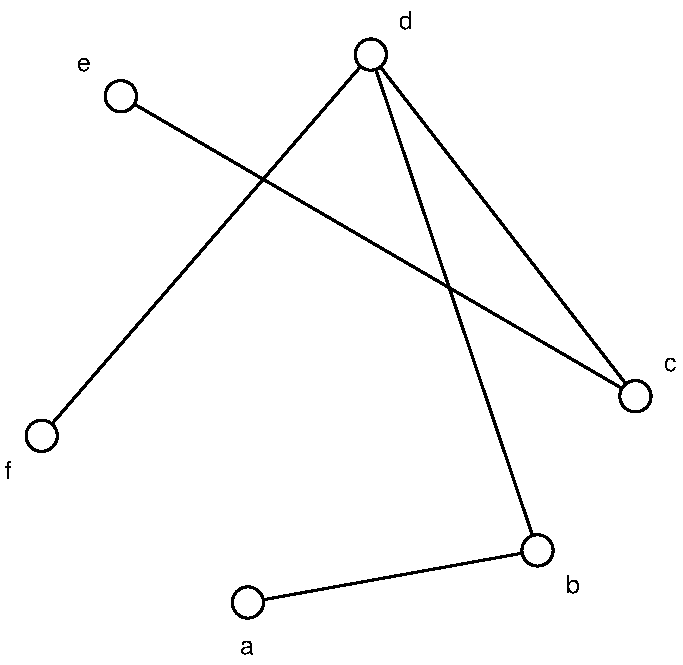
\includegraphics[width=\textwidth]{img/example_conflict_graph_segments.pdf}
          \caption{Line Segments}
  \end{subfigure}
  \hspace{2em}
  \VRule
  \hspace{2em}
  \begin{subfigure}{0.4\textwidth}
          \centering
          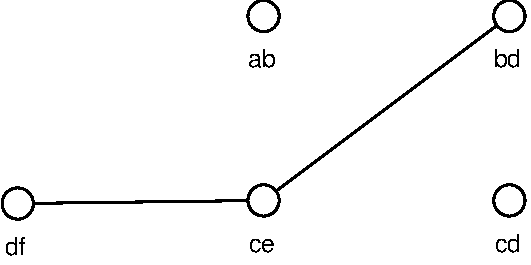
\includegraphics[width=\textwidth]{img/example_conflict_graph.pdf}
          \caption{Conflict Graph}
  \end{subfigure}  
  \caption{\label{fig:example_conflict_graph}Example of the Conflict %
    Graph for a given set of line segments %
    and the conflicts being all intersections}
\end{figure}

Now we can combine the previous definitions to characterize
triangulations. Note that we start off with a combinatorial
definition without any geometric components. In the course of this
chapter, we show how to apply this formulation to geometric problems.

\begin{definition}[Triangulation]
  Given the Complete Graph \(K_V = (V,E)\) for a vertex set \(V\)
  and a set of conflicts \(X\) for \(E\)
  such that the Conflict Graph \(\gls{Gconf}[(E,X)]\) is \gls{wcover}.
  A \emph{Triangulation} \(T(V,X) \subseteq E\) of \(V\) with respect
  to \(X\) is a maximum set of non-conflicting edges:
  \[
    e_i \in T(V,X)
    \iff e_i \in E
    \land \forall e_j \in T(V,X) : \{e_i,e_j\} \not\in X
  \]
\end{definition}

Bringing the Maximum Independent Set from \cref{sec:independent_set}
back to mind, we can see that a Triangulation is essentially the same
problem. Apart from Triangulations operating on the Conflict Graph,
both problems maximize the number of ``independent'' vertices.

\begin{theorem}[Equality of Triangulation and Maximum Independent Set]
  \label{thm:triangulation_independent_set}
  Every Triangulation \(T(V,X)\) of a vertex set \(V\) with respect
  to conflicts \(X\) is a Maximum Independent Set for the Conflict
  Graph \(\gls{Gconf}[(E,X)]\) and vice versa. Hereby \(E\) are the
  edges of the Complete Graph \(K_V\).
  \begin{proof}
    \Cref{thm:triangulation_independent_set} follows directly from
    \cref{def:max_independent_set,thm:well_covered_independent_set}.
  \end{proof}
\end{theorem}

Now we can make use of \cref{alg:greedy_independent_set} from
\cref{cha:integer_programming} to gain a first bound on the time
complexity of finding \emph{any} Triangulation (for a given vertex
set and conflicts). Later, we give more accurate time bounds for
special classes of Triangulations.

\begin{theorem}[Time Complexity of Triangulations]
  \label{thm:time_complexity_triangulations}
  From
  \cref{%
    thm:triangulation_independent_set,%
    thm:well_covered_maximum_independent_set%
  }
  follows that finding a Triangulation \(T(V,X)\) of a vertex set
  \(V\) with respect to conflicts \(X\) takes \(O(|X|)\) time.
\end{theorem}

One important property of geometric objects has not been considered
for our definition of Triangulations yet: \emph{forbidden objects}.
Besides conflicting objects
from which only one can be part of the same Triangulation, there may
as well be objects which are not wanted at all---as we consider the
Complete Graph. This can be the case when a Triangulation is required
to lie completely within a certain boundary or when one object
overlaps multiple others.

\begin{definition}[Triangulation with Forbidden Edges]
  \label{def:triangulation_forbidden_edges}
  A \emph{Triangulation with Forbidden Edges} \(T(V,X,F)\) is a 
  Triangulation of the vertex set \(V\) with respect to conflicts
  \(X\) which does not contain any of the edges in \(F\):
  \[ \forall e \in F : e \not\in T(V,X,F) \]
\end{definition}

Even though this \namecref{def:triangulation_forbidden_edges} models
geometric triangulation problems better, it is not solvable in
polynomial time anymore (assuming P\(\not=\)NP). Many geometric
triangulations are solvable in polynomial time however (as we see
later)---so this approach is clearly not the best one to solve them.

\begin{theorem}[NP-completeness of Triangulation with Forbidden Edges]
  The decision problem whether 
  a Triangulation with Forbidden Edges \(T(V,X,F)\) exists
  is NP-complete.
  \cite[triangulation existence problem]{triangulation_forbidden_edges}
\end{theorem}

There is another approach to ensure that boundary is part of a
Triangulation which we call \emph{constraints}. Basically we require
a Triangulation to contain certain objects, e.g. the boundary. This
leaves the problem that objects outside the boundary can be part of
the Triangulation but those can be removed from the Triangulation
in polynomial time (because triangulations have polynomial size).

\begin{definition}[Constrained Triangulation]
  \label{def:constrained_triangulation}
  A \emph{Constrained Triangulation} \(T(V,X,C)\) is a Triangulation
  of the vertex set \(V\) with respect to conflicts \(X\) which 
  contains the edge constrains \(C\):
  \[ \forall e \in C : e \in T(V,X,C) \]
\end{definition}

In contrast to the Triangulation with Forbidden Edges, Constrained
Triangulations can be found in polynomial time. Therefore we slightly
modify \cref{alg:greedy_independent_set} to begin with the constraints
as initial Independent Set and then proceed as before. This assumes
that the constraints themselves are all valid and not conflicting.
Even without that guarantee, an additional check before running the
algorithm would require at most quadratic time with respect to the
constraints---so the whole running time is still polynomial.

\begin{theorem}[Time Complexity of Constrained Triangulations]
  Using \cref{alg:greedy_independent_set}
  a Constrained Triangulation \(T(V,X,C)\) of the vertex set \(V\)
  with respect to conflicts \(X\) and constrains \(C\)
  can be calculated in \(O(|C|^2 + |X|)\) time.
  In case \(C\) is guaranteed to have the Independent Set property,
  running time reduces to \(O(|X|)\).
\end{theorem}

\section{Point Set Triangulations}
\label{sec:point_set_triangulations}
In this \namecref{sec:point_set_triangulations} we present the first
geometric triangulation problem and draw the connection to our
previous definition. The difference between a (topological)
Triangulation as we have defined it earlier and a Point Set
Triangulation which we get to in this
\namecref{sec:point_set_triangulations} can be seen as the distinction
between a graph and its embedding.

To make things clear, we start by defining some geometric terms which
we use in the following. The equivalent of edges in a topological
triangulation are line segments for a geometric triangulation in the
plane. Since line segments are not restricted to the plane, we do not
focus on two dimensions here. However according to some definitions,
triangulations for higher dimensions contain also geometric objects
of higher dimension (e.g. tetrahedra in three dimensions). For
simplicity we consider those objects be implicitly defined by their
bounding line segments.

% \begin{definition}[Planar Points]
%   A \emph{planar set of points} or \emph{set of points in the plane}
%   \(P\) is a set of points with two coordinates:
%   \[ P \subseteq \{p = (p_x,p_y) : p_x,p_y \in F\} \]
%   We do not make any assumptions on the coordinates besides \(F\)
%   being a field, e.g. the real numbers \gls{R}. Furthermore,
%   because \(P\) is a set, no duplicate points \(p=(p_x,p_y)\in P\) and
%   \(p'=(p_x',p_y')\in P\) with \(p_x=p_x'\) and \(p_y=p_y'\) are allowed.
%   Note however that we do not require the points in \(P\) to be in 
%   general position as that would forbid some interesting instances.
%   \todo[inline]{do we need this definition at all?}
% \end{definition}

\begin{definition}[Line Segments]
  A \emph{line segment} \(s=(p,q)\) is determined by its endpoints
  \(p,q\in P\) with \(P\) being a point set (of arbitrary dimension). 
  For compatibility with other definitions,
  \(s\) is directed from \(p\) to \(q\), i.e. \((p,q)\not=(q,p)\)
  and contains all points ``between'' \(p\) and \(q\):
  \[ m \in s \iff \exists a\in [0,1] : m = p + a \cdot (q-p) \]
\end{definition}

Clearly, counterpart of conflicting edges are intersecting line
segments. Nevertheless, depending on the definition, intersection of
two line segments with the same endpoint is empty or the common endpoint.
This is why we assume intersection of any geometric objects to be the
set intersection of all (usually infinitely many) points contained in
the objects and introduce the already widely used term \gls{cross}:

\begin{definition}[Crossing]\label{def:crossing}
  Two line segments \(s_i=(p_i,q_i)\) and \(s_j=(p_j,q_j)\) with 
  different slope are \gls{cross}, if their intersection is not empty
  and not an endpoint, i.e.
  \[
    s_i, s_j~\gls{cross}
    \iff
    (p = s_i\cap s_j) \land
    (|s_i\cap s_j| = 1) \land
    (p \not\in \{p_i,q_i,p_j,q_j\})
  \]

  Two line segments \(s_i\) and \(s_j\) are \gls{ncross}
  if they are not \gls{cross}.
  A set \(S\) of line segments is \gls{cross}
  if at least two segments \(s_i, s_j \in S\) are \gls{cross}.
  It is \gls{ncross} if each pair \(s_i, s_j \in S\) is \gls{ncross}.
\end{definition}

We do not require points to be in general position which is why we
have to deal with degeneracies in the following. General position
often preempts interesting instances---e.g. those which are heavily
symmetric. Additionally, many man-made structures aim for
collinearity, so extra effort has to be expended to make real world
instances fit the general position requirements. The following
\namecref{def:overlapping_segments} identifies all unwanted line
segments in case of collinear points. Refer to
\cref{fig:overlapping_segments} for examples of such degeneracies.

\begin{definition}[Overlapping Line Segments]
  \label{def:overlapping_segments}
  Given a point set \(P\) and a line segment \(s = (p,q)\) with
  \(p,q \in P\). \(s\) is \gls{overlap} in \(P\) if and only if
  there is a point \(p' \in P\) which lies in its interior:
  \[
    s~\gls{overlap}
    \iff  \exists p' \in P : (p' \in s) \land (p' \not\in \{p,q\})
  \]
  \(s\) is \gls{noverlap} if it is not \gls{overlap}.
\end{definition}

\begin{figure}[ht]
  \centering
  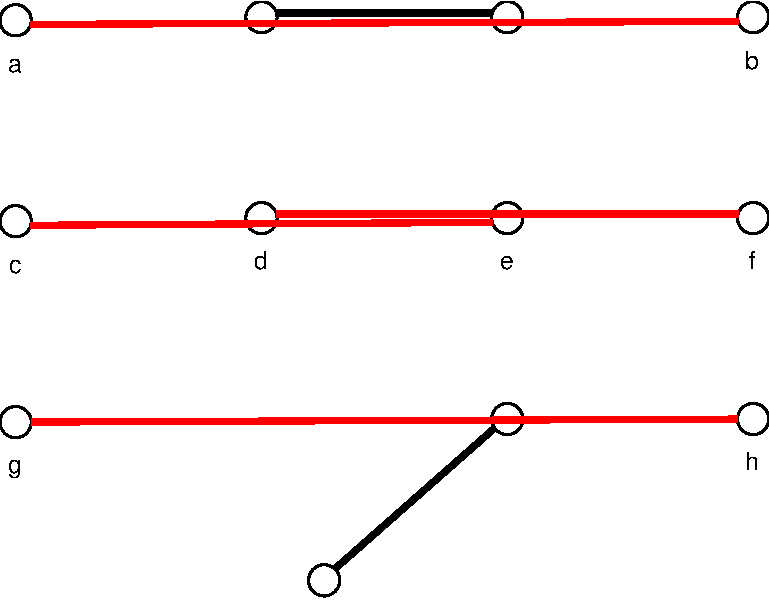
\includegraphics[width=0.5\textwidth]{img/example_overlapping.pdf}
  \caption{\label{fig:overlapping_segments}%
    Examples of overlapping line segments %
    (\(\{a,b\}, \{c,e\}, \{d,f\}, \{g,h\}\))%
  }
\end{figure}

Earlier in this \namecref{sec:point_set_triangulations}, we already
mentioned the connection between topological and geometric
triangulations---and here comes the formal definition. Note that
we distinguish between points (which have a geometry, i.e.
coordinates) and vertices (which are solely topological objects).

\begin{definition}[Topological Representation]
  A vertex set \(V(P)\) \emph{represents} a point set \(P\) if there
  is exactly one vertex \(v_p \in V(P)\) for each point \(p \in P\)
  and \(v_p\) can be identified by \(p\) and vice versa.
%   
%   An edge set \(E(S)\) represents a set of line segments \(S\) iff
%   there is exactly one edge \(e_s = \{v_p, v_q\} \in E(S)\) for each 
%   line segment \(s = (p,q) \in S\) and \(e_s\) can be identified by
%   \(s\) and vice versa. The endpoints \(p\) and \(q\) of \(s\) are 
%   represented by the vertices \(v_p\) and \(v_q\), respectively. We
%   hereby assume that not \((p,q) \in S\) and \((q,p) \in S\) as they
%   would be represented by the same edge.
\end{definition}

After having all basic terms at hand, we now proceed with
\emph{Point Set Triangulations}. They are the geometric equivalent
of topological triangulations for point sets. To emphasize that
Point Set Triangulations without further restrictions can be 
calculated in polynomial time (compare
\cref{thm:time_complexity_triangulations,%
  thm:time_complexity_planar_point_set_triangulations}),
we avoid the definition to be based on 
Triangulations with Forbidden Edges (see
\cref{def:triangulation_forbidden_edges})---despite the fact that
overlapping line segments are forbidden edges. Note in this case that
finding a Triangulation involving overlapping line segments takes
polynomial time. Afterwards they can be replaced by the line segments
that they include in polynomial time (because there are polynomially
many line segments).

\begin{definition}[Point Set Triangulation]
  \label{def:point_set_triangulation}
  The Triangulation \(T(P)\) of a point set \(P\)
  is a triangulation \(T(P) = T(V,X)\)
  where the vertex set \(V=V(P)\) represents \(P\), 
  the conflicts \(X\) are all \gls{cross} line segments, 
  and which contains no \gls{overlap} line segments:
  \begin{alignat*}{1}
    (p,q), (p',q')~\gls{cross}
    &\iff \left\{ \{v_p,v_q\}, \{v_{p'},v_{q'}\} \right\} \in X \\
     (p,q)~\gls{overlap}
    &\implies \{v_p,v_q\} \not\in T(P)
  \end{alignat*}

  For convenience we define \(s=(p,q) \equiv e=\{v_p,v_q\}\) such
  that \(s \in T(P) \iff e \in T(P)\). See also
  \cite[Section 9.1]{deberg_compgeom} for a slightly different yet
  equivalent definition of Point Set Triangulations.
\end{definition}

The asymptotic time complexity of finding a Triangulation can be 
improved for the special case of Point Set Triangulations. For example
by making use of sweep line algorithms which exploit that
Triangulation properties can be ensured locally, the running time
drops to \(O(n \log n)\)---as in \cite{fortunes_algorithm}.

\begin{theorem}[Time Complexity of Planar Point Set Triangulation]
  \label{thm:time_complexity_planar_point_set_triangulations}
  A planar point set \(P \subseteq \gls{R}[^2]\) can be triangulated
  in \(O(n \log n)\) time with \(n = |P|\).
  \cite[Theorem 9.12]{deberg_compgeom}
\end{theorem}

In \cref{def:constrained_triangulation} we already showed a way to
force certain objects (e.g. boundaries) to be part of a Triangulation.
The same concept can be transferred to Point Set Triangulations as in
the following \namecref{def:constrained_point_set_triangulation}:

\begin{definition}[Constrained Point Set Triangulation]
  \label{def:constrained_point_set_triangulation}
  A \emph{Constrained Point Set Triangulation} \(T(P,C)\)
  of a point set \(P\) with line segment constraints \(C\)
  is a Point Set Triangulation \(T(P,C) = T(P)\)
  such that \(C \subseteq T(P, C)\).
\end{definition}

The same time bound holds in the presence of constraints. Sweep line 
algorithms can be modified for taking constraints into account. Note
that constraints can destroy desired properties of a Point Set
Triangulation (such as large inner angles)---we come back to some of
those additional requirements later in this
\namecref{cha:triangulations}.

\begin{theorem}[Constrained Point Set Triangulation]
  A \emph{Constrained Point Set Triangulation} \(T(P, C)\)
  for a planar point set \(P \subseteq \gls{R}^2\)
  and line segment constraints \(C \subseteq P^2\)
  can be calculated in \(O(n \log n)\) time.
  \cite{constrained_triangulation}
\end{theorem}

\section{Intersection Graph}
\label{sec:intersection_graph}

%---------------------------------------------------------------------##########
\todo[inline]{glue text}


\begin{definition}[Intersection Graph]
  \label{def:intersection_graph}
  For a set of line segments \(S\) the \emph{intersection graph}
  \(\gls{Gcross}[(S)] = (V_S,X)\) consists of a vertex \(v_s \in V_S\)
  for every line segment \(s \in S\) and an edge
  \(\{v_{s_i}, v_{s_j}\} \in X\) for every pair of \gls{cross}
  segments \(s_i, s_j \in S\). It is the geometric equivalent of the
  conflict graph (\cref{def:conflict_graph}).
\end{definition}

\todo[inline]{glue text}

\begin{theorem}[Computational Complexity of Intersection Graph]
  \label{thm:sweep_bound}
  Given a set of line segments \(S\) the intersection graph
  \(\gls{Gcross}[(S)] = (V_S,X)\) can be calculated in
  \(O(m \log m + i \log m)\) time where \(m = |V_S| = |S|\) 
  and \(i = |X|\) is the number of intersections in \(S\).
  \cite[Lemma 2.3]{deberg_compgeom}
\end{theorem}

\todo[inline]{glue text}

\begin{theorem}[Complexity of Point Set Intersections]
  \label{thm:point_set_intersections}
  For a point set \(P\) with \(n\) points the set of all line 
  segments \(S\) with endpoints in \(P\) has \(\Theta(n^4)\) 
  intersections. \cite{quadrilaterals_bound} Thus calculating the
  intersection graph for \(S\)  takes \(\Omega(n^4)\) time.
\end{theorem}

\todo[inline]{glue text}

\begin{theorem}[Non-Optimality of Sweep Algorithm for Point Sets]
  The sweep algorithm presented in \cite[Section 2.1]{deberg_compgeom}
  with the time complexity of \cref{thm:sweep_bound} is not optimal
  for calculating the intersections of all line segments with
  endpoints in a given point set \(P\) as it takes \(O(n^4 \log n)\)
  time.
\end{theorem}

\todo[inline]{glue text}

\begin{algorithm}
  \DontPrintSemicolon
  
  \KwIn{Set of segments \(S\)}
  \KwOut{Intersection graph \(\gls{Gcross}[(S)] = (V_S,X)\)}
  
  Set \(V_S = \{v_s : s \in S\} \) \;
  Set \(X = \emptyset\) \;
  \ForEach{\(s \in S\)}{
    \ForEach{\(\gls{scross} \in S\) with \(|s| \leq |\gls{scross}|\)}{
      \If{\(s\) and \gls{scross} are \gls{cross}}{
        Add \(\{v_s, v_{\gls{scross}}\}\) to \(X\) \;
      }
    }
  }
  \KwRet{\(\gls{Gcross}[(S)] = (V_S,X)\)}
  \caption{\label{alg:naive_intersection}Naive Intersection Algorithm}
\end{algorithm}

\todo[inline]{glue text}

\begin{theorem}[Complexity and Correctness of \Cref{alg:naive_intersection}]
  \Cref{alg:naive_intersection} finds all intersecting line segments
  in \(O(m^2)\) time with \(m = |S|\).  
\end{theorem}

\todo[inline]{glue text}

\begin{theorem}[Optimality of \Cref{alg:naive_intersection} for Point Set]
  \Cref{alg:naive_intersection} is asymptotically optimal for finding
  the intersections of all line segments with endpoints in a given
  point set \(P\) as it takes \(O(n^4)\) time for \(n = |P|\).
\end{theorem}

%---------------------------------------------------------------------##########

% One day Greg had art class and the children were given sheets of
% paper with points on them. The task was to connect all the points 
% such that they have as many bounded areas as possible. Greg 
% connected all the points taking care that the connections would only 
% intersect in the given points. He was happy to see that the result 
% consisted only of triangles filling up the whole space within the 
% points. Also he had more bounded areas than any other child --- 
% even more than Joey who filled up his sheet with quadrangles. Greg's
% teacher, Mrs. Minerva, told him that he made a triangulation.
% 
% After seeing Greg's sheet, some of his friends let their connections
% cross each other to get more areas, but Greg considered that
% cheating. To stay the winner of the competition he made a new rule
% that no point connections are allowed to cross.
% 
% Joey tried to circumvent Greg's rule by adding new points to his
% sheet. For each new point he added on the outside he could make
% several new connections and therefore got soon many more areas. So
% Greg had to quickly come up with another rule only allowing the
% existing points to take part of the competition.
% 
% \begin{definition}[Induced Segments]\label{def:induced_segments}
%   The set of induced line segments \(S_P\) of a planar point set \(P\)
%   consists of all \gls{noverlap} unique line segments having
%   endpoints in \(P\):
%   \[
%     S_P := \{s=(p,q) \in P^2 : (p < q) \land s~\gls{noverlap}\}
%   \]
%   Let \(<\) hereby denote the lexicographical order, that is for
%   \(p = (p_x,p_y)\) and \(q = (q_x,q_y)\):
%   \[
%     p < q \iff (p_x < q_x) \lor ((p_x = q_x) \land (p_y < q_y)).
%   \]
% \end{definition}
% 
% With those two new rules no one could think of a better way to make
% areas than Greg's triangles. Even Mrs. Minerva said that under those
% conditions it would not be possible to come up with a subdivision
% which has more faces than a triangulation.
% 
% \begin{verbatim}
%   - observation: when changing geometry but not topology,
%     certain properties stay the same
%   - e.g. angle/area/length preserving transformation
%     => many optimal triangulations map to one topological
%     (size doesn't matter)
% \end{verbatim}
% \todo[inline]{notes}

\section{Polygon Triangulations}

\todo[inline]{glue text}

\begin{definition}[Polygon Triangulation]
  A triangulation \(T(P)\) of a polygon \(P\) bounded by line segments
  are all boundary and interior edges of \(P\) in a constrained point
  set triangulation of the polygon vertices with the polygon boundary
  as constraints.
\end{definition}

\todo[inline]{glue text}

\begin{theorem}[Generalization of Point Set Triangulation]
  Given a point set \(P\), a triangulation \(T(\conv(P) \cup P)\) of
  the polygon bounded by the convex hull \(\conv(P)\) of \(P\) and
  containing all inner points of \(P\) is a triangulation of \(P\).
\end{theorem}

\section{Edge Flipping}

\todo[inline]{glue text}

\begin{definition}[Edge Flip]
  \label{def:edge_flip}
  Given a triangulation \(T(V,X)\) for a vertex set \(V\) with respect
  to a set of conflicts \(X\), \((e, f)\) with \(e \in T(V,X)\) and
  \(f \not\in T(V,X)\) is an \emph{edge flip} iff
  \(T(V,X) \setminus \{e\} \cup \{f\}\) is a triangulation for \(V\)
  with respect to \(X\).
\end{definition}

\todo[inline]{glue text}

\begin{theorem}[Edge Flips are Conflicts]
  Given a triangulation \(T(V,X)\) for a vertex set \(V\) with respect
  to a set of conflicts \(X\), every edge flip \((e,f)\) is a
  conflict: \(\{e,f\} \in X\).
\end{theorem}

\begin{proof}
  Assume \(\{e,f\} \not\in X\). Further assume that
  \[ \lnot\exists e' \in T(V,X)\setminus\{e\}: \{e', f\} \in X. \]
  Then \(f\) can be added to \(T(V,X)\) (without removing \(e\)) and
  therefore \(T(V,X)\) is no triangulation---which is a 
  contradiction. Now let \(e' \in T(V,X)\setminus\{e\}\) such that
  \(\{e', f\} \in X\). Then \(e' \in T(V,X)\setminus\{e\} \cup f\)
  ---which contradicts that \(T(V,X)\setminus\{e\} \cup f\) is a
  triangulation. Therefore every edge flip \((e,f)\) is a conflict.
\end{proof}

\todo[inline]{glue text}

\begin{definition}[Flip Graph]
  \label{def:flip_graph}
  The flip graph \(\gls{Gflip}[(V,X)] = (V_T,\gls{Eflip})\) for a
  vertex set \(V\) and edge conflicts \(X\) contains a vertex
  \(v \in V_T\) for every triangulation of \(V\) with respect to
  \(X\) and edges \(e \in \gls{Eflip}\) for every possible edge flip.
\end{definition}

\todo[inline]{glue text}

\begin{figure}[ht]
  \centering
  \begin{subfigure}{0.3\textwidth}
    \centering
    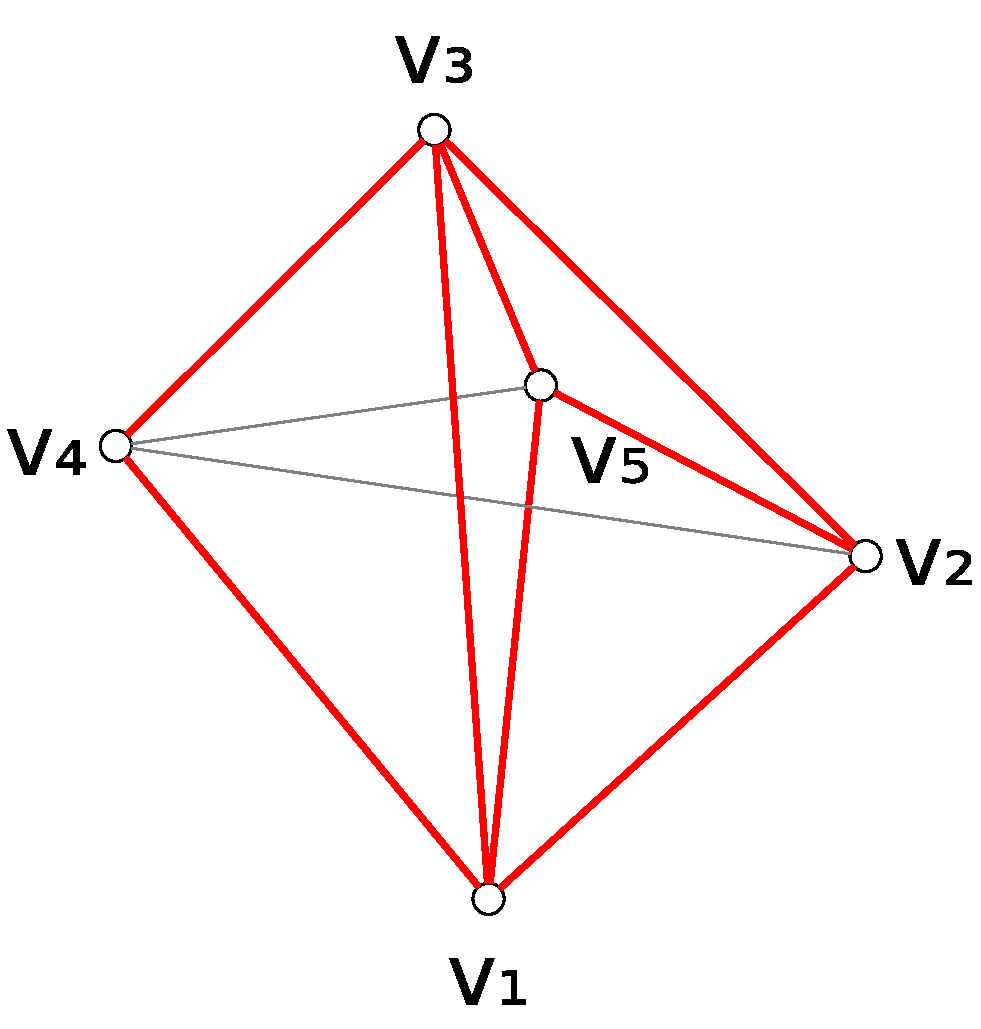
\includegraphics[width=\textwidth]{img/example_triangulation_1.pdf}
    \caption{}
  \end{subfigure}
  \hspace{0em}
  \VRule
  \hspace{0em}
  \begin{subfigure}{0.3\textwidth}
    \centering
    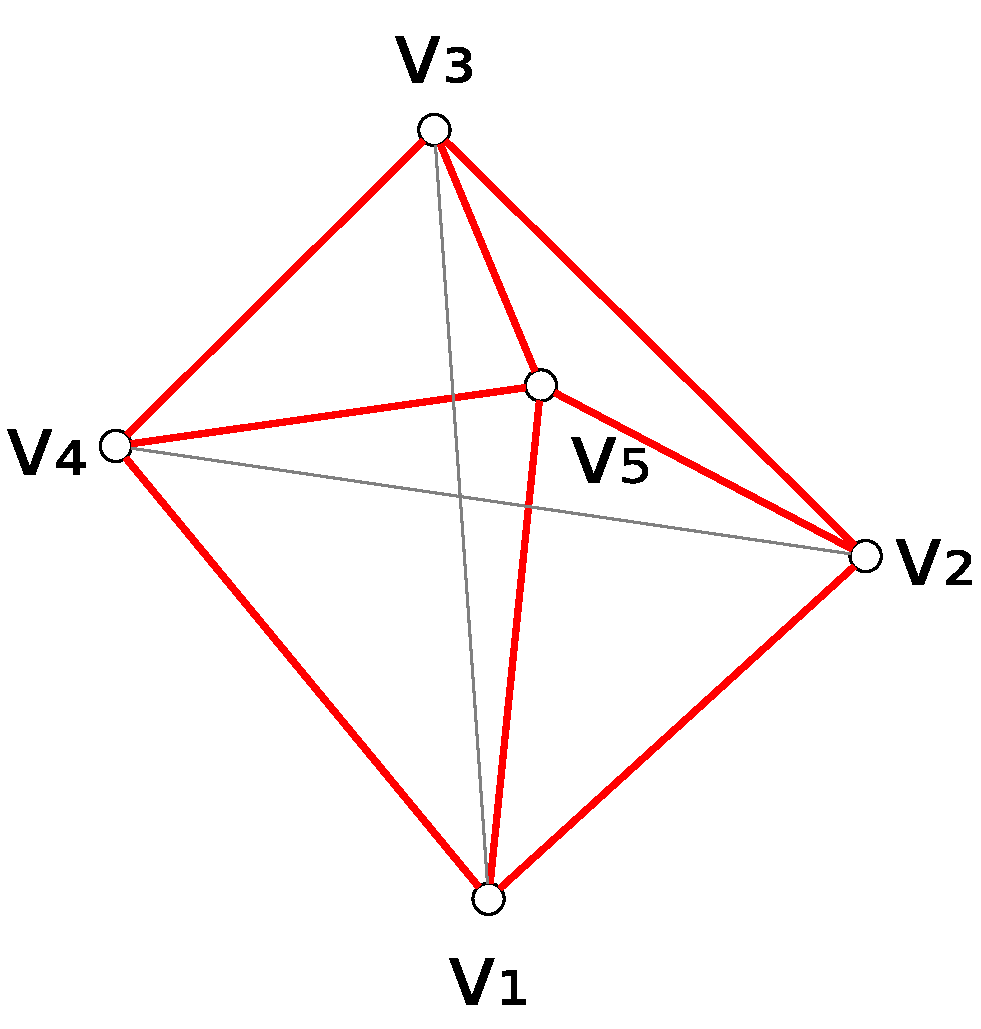
\includegraphics[width=\textwidth]{img/example_triangulation_2.pdf}
    \caption{}
  \end{subfigure}
  \hspace{0em}
  \VRule
  \hspace{0em}
  \begin{subfigure}{0.3\textwidth}
    \centering
    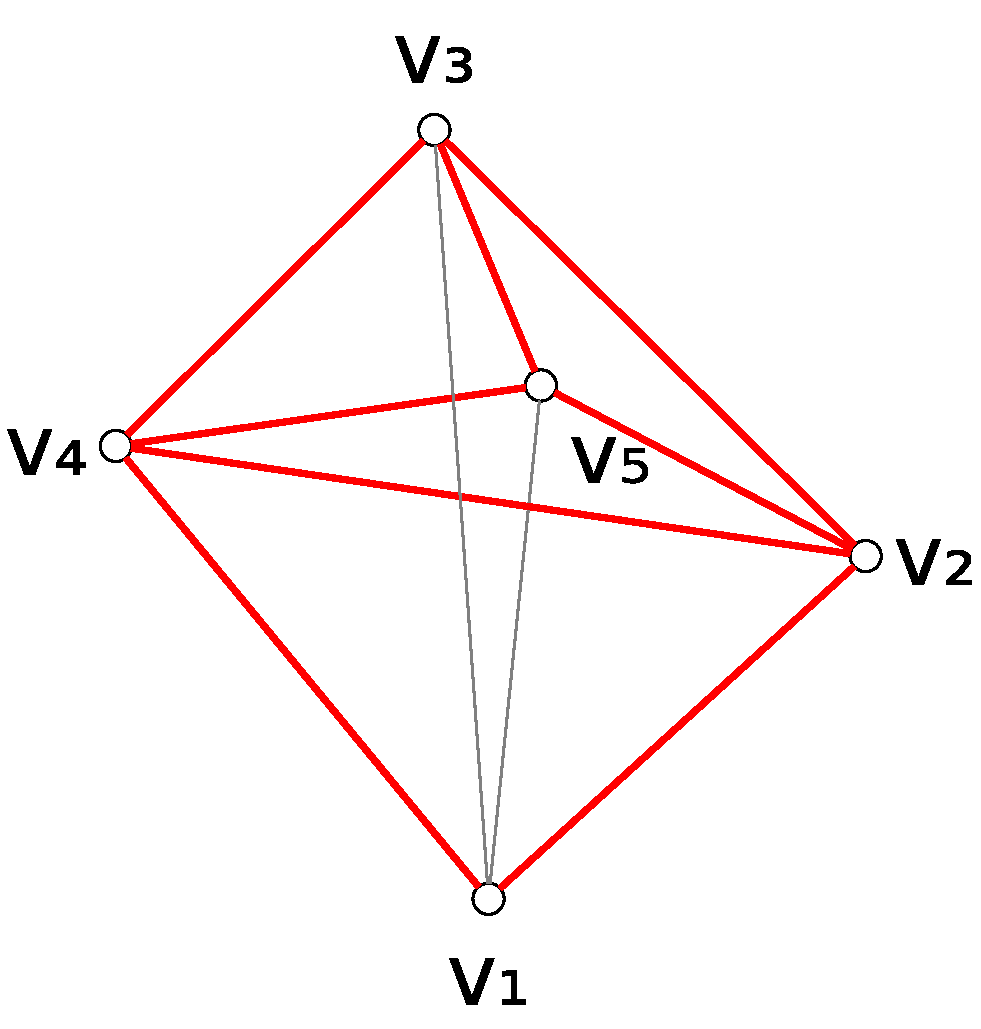
\includegraphics[width=\textwidth]{img/example_triangulation_3.pdf}
    \caption{}
  \end{subfigure}
  
  \vspace{2em}
  \begin{subfigure}{0.7\textwidth}
    \centering
    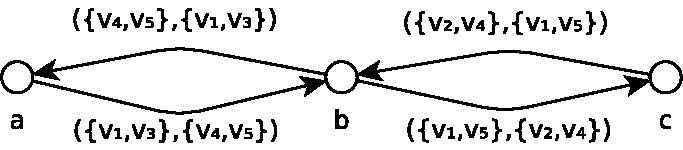
\includegraphics[width=\textwidth]{img/example_flip_graph.pdf}
  \end{subfigure}
  \caption{Example triangulations and their flip graph}
\end{figure}

\todo[inline]{glue text}

\begin{theorem}[Connectivity of the Flip Graph]
  The flip graph \(\gls{Gflip}[(V,X)]\) is connected in two dimensions
  \cite[Behauptung 4]{flip_graph_connected} and has a diameter of
  at most \(6n - 30\) for \(n = |V|\).~\cite{flip_graph_diameter}
  Therefore every triangulation \(T(V,X)\) of a vertex set \(V\)
  with respect to edge conflicts \(X\) can be transformed into any
  other triangulation of \(V\) with respect to \(X\) in \(O(n)\)
  time.
  
  For three dimensions, it is still an open problem whether
  the flip graph is connected.~\cite{flip_graph_3d}
\end{theorem}

\begin{verbatim}
  - local vs. global optimal
  - hint to edge flipping paper
\end{verbatim}
\todo[inline]{notes}

%---------------------------------------------------------------------##########

\section{Related Work}
After class was over, Greg asked Mrs. Minerva if there are different
kinds of triangulations. She replied that the problem of 
triangulating has kept researchers busy for over 100 years already
\cite{triangulation_hilbert} and that people have found different
aspects in that a triangulation can be optimal.

The most famous class is the Delaunay triangulation
\cite[Section 9.2]{deberg_compgeom}. It forces every circumcircle
of a triangle to be empty of other points and therefore maximizes
the minimum angle \cite[Theorem 9.9]{deberg_compgeom}. There is an
edge flipping algorithm which calculates it in \(O(n \log n)\) 
expected time using \(O(n)\) space 
\cite[Theorem 9.12]{deberg_compgeom}.

There are several other triangulations which can be computed in
polynomial time. Minimizing the maximum edge length in \(O(n^2)\)
times was one of the first results \cite{triangulation_minmax_length}.
The counterpart of a Delaunay triangulation, 
minimizing the maximum angle, takes \(O(n^2 \log n)\) time and
\(O(n)\) space \cite{triangulation_edge_insertion}. The same
approach can also produce triangulations which maximize the minimum 
height of a triangle. Finally, the same reference shows also that 
minimizing the maximum slope and minimizing the maximum eccentricity 
can both be done in \(O(n^3)\) time and \(O(n^2)\) space. A 
triangulation which minimizes or maximizes the area of triangles can
be computed in \(O(n^2 \log n)\) time with \(O(n^2)\) space.
\cite{triangulation_area}

Other triangulations have been proven NP-hard or NP-complete. One
of them is to minimize the edge length sum (also known as the minimum
weight triangulation) which is NP-hard \cite{mwt_complexity}. 
Maximizing the minimum edge length was stated an open problem
\cite{triangulation_minmax_length} but 20 years later it has been
shown that it is NP-complete \cite{mmlt_complexity}. The latter one
remains NP-hard for polygons with holes and interior points
\cite{mmlt_polygons} but can be solved in \(O(n^3)\) time for simple
polygons and even in linear time for convex polygons
\cite{mmlt_convex_polygons}.

%---------------------------------------------------------------------##########
